\documentclass[a4paper, 12pt]{article}
    \usepackage[portuges]{babel}
    \usepackage[utf8]{inputenc}
    \usepackage{amsmath}
    \usepackage{indentfirst}
    \usepackage{graphicx}
    \usepackage{placeins}
    \usepackage{multicol,lipsum}
    \usepackage{indentfirst}
    \usepackage[nottoc,notlot,notlof]{tocbibind}
    \setlength{\parindent}{0.6cm}
    \newcommand\tab[1][0.6cm]{\hspace*{#1}}
    
        
        
    \begin{document}
    \sloppy
    \begin{titlepage}
      \begin{center}
          \Huge{Universidade Federal de Pernambuco}\\
          \large{Deep Logic Networks: Inserting and Extracting
    Knowledge From Deep Belief Networks}\\ 
          \vspace{15pt}
          \vspace{95pt}
          \textbf{\LARGE{Relatório}}\\
          \vspace{3,5cm}
      \end{center}
    
      \begin{flushleft}
          \begin{tabbing}
                      José Nilton\\
                      Italo Paulino\\
                      Mateus Gonçalves\\ 
                      Wallace Soares\\
          \end{tabbing}
      \end{flushleft}
      \vspace{1cm}
    
      \begin{center}
          \vspace{\fill}
          Junho - 2018\\
      \end{center}
    \end{titlepage}
    \newpage
    \tableofcontents
    \thispagestyle{empty}
    \newpage
    \pagenumbering{arabic}
    \section{Introdução}
    O uso de redes \textit{deep} para resolução de problemas complexos envolvendo \textit{Big Data} vem sendo cada vez mais comum nas ultimas décadas. Entretanto compreender o treinamento deste tipo de rede não é trivial. Áreas como a \textit{neural-symbolic computing} estudam em como o conhecimento pode ser inserido e extraido de redes neurais \textit{deep} \cite{Tran}, \cite{garbook}, \cite{garConf}. Através da inserção de conhecimento Tran e Garcez \cite{Tran} mostraram que é possível economizar tempo de processamento pois tal inserção já será uma alternativa a fase de pré-treinamento.
    Já a extração de conhecimento é importante por duas razões: compreensão e re-inserção de conhecimento. Compreender como cada unidade da rede esta aprendendo o padrão de entrada. Re-inserção pois uma vez em que sabemos como cada unidade aprendeu a reproduzir o padrão de entrada podemos modificar o conhecimento da rede para obter um melhor seu treinamento.
    
    Tran e Garcez\cite{Tran} propõem no artigo em análise um método de inserção e extração de conhecimento em \textit{Deep Belief Networks} - DBNs. DBNs são definidas como n-Restricted Boltzman Machines - RBMs empilhadas de forma que a camada de escondida de uma RBM seja a camada visivel da próxima como mostra a figura abaixo. Exploramos os conceitos de RBMs e DBNs nas seções 1.1 e 1.2, respectivamente.
    
    \begin{figure}[h]
     \centering
     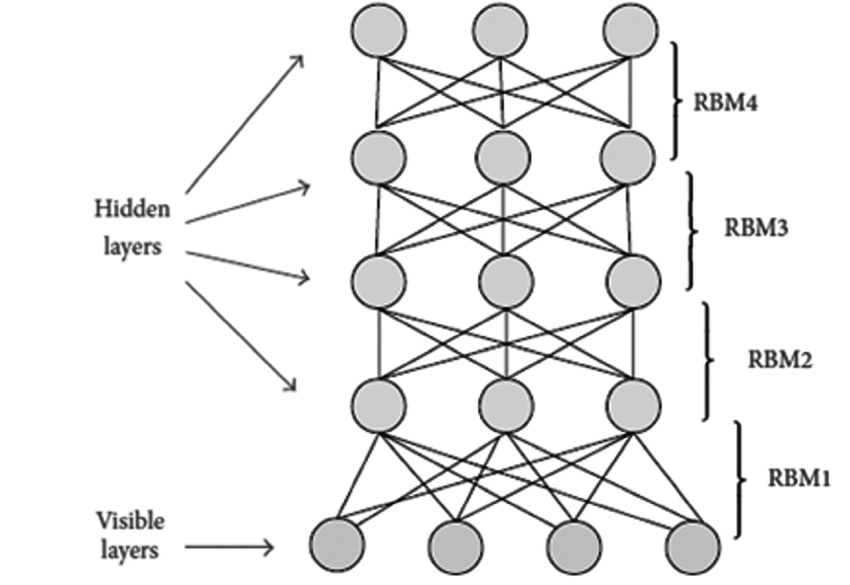
\includegraphics[scale=0.3]{Graphical-Representation-of-a-Deep-Belief-Network.png}
     \caption{Representação gráfica de \textit{Deep Belief Networks}.\cite{imagem1}}
    \end{figure}
    
    \subsection{Restricted Boltzman Machines}
    RBMs constituem-se por neurônios ligados por grafos bidirecionais que conectam a camada visivel à camada escondida. O objetivo desta rede é aproximar ao máximo o resultado da camada escondida com o que esta sendo apresentado na entrada. Através da apresentação do padrão de entrada na camada visivel, RBMs criam padrões numéricos na camada escondida que estão diretamente relacionados com os pesos das areastas e com as funções de ativação. A partir dos padrões numéricos, a camada escondida tenta reconstruir na camada visível o que foi apresentado como entrada. Este processo é repetido até que a RBMs produza com maior acurácia o padrão de entrada. Apesar dessa caracterista de automaticamente detectar padrões, RBMs podem ser utilizadas tanto para aprendizado supervisionado ou não-supervisionado. Como definido por \cite{overviewRBM}, RBMs são modelos baseados em energia, isto é para cada estado que a RBM possuir, uma energia será associada e assim um probalidade da rede estar representando o padrão de entrada.
    \subsection{Deep Beliefs Networks}
    DBNs são essencialmente várias RBMs empilhadas em que a camada escondida de uma RBM será a camada visível da próxima, e assim sucessivamente. Ao contrário dos \textit{Convolutional Neural Networks}(CNNs) que precisam dados previamente categorizados para o treinamento, DBNs utilizam as RBMs para reproduzir o padrão de entrada camada por camada. Como proposto por Hinton\cite{Hinton} o primeiro passo para o treinamento de uma DBN é usar o algoritmo \textit{contrastive divergence}(CD) para reproduzir as principais \textit{features} de entrada na primeira camada visivel. Após este passo, estas features serão utilizadas como entrada na segunda RBM, como entrada. Este processo é repetido até que a ultima camada finalize seu treinamento. Entretanto, após a ultima camada finalizar seu treinamento ainda não se sabe como comparar a saida da DBN com dados reais. Para isso utiliza-se algoritmos de aprendizado supervisionado que categoriza a saida da DBNs, identificando os dados com o conjunto de dados utilizado.  
    
    \subsection{Regras de Confidência}
    Como definido em \cite{Tran}, regras de confidência são formulas bicondicionais(se, somente se) como indicado abaixo:
    
    \begin{equation}
    c : h \leftrightarrow x_1 \wedge ... \wedge x_n
    \qquad \text{Regra de Confidência}
    \end{equation}
    
    Onde $h$ é uma proposição atomica e cada $x_i$ é um literal(uma proposição atômica ou sua negação), classificadas por um valor real $c$ chamado de valor de confidência. As regras de confidência serão utilizadas tanto na extração, como na inserção de conhecimento.
        
    \section{Módulos}
    
    Esta seção aborda os principais componentes da implementação que são a inferência, a extração e inserção de regras de confidência.
    \subsection{Inferência}
    As regras de confidência também podem ser classificadas por hierarquias\cite{Tran}. Isto é, utilizar uma regra base que possua todos os valores de confidência da entrada para inferir um sub-conjunto de regras que possuem valores de confidencia distintos. Assim é possível encontrar qual regra possui uma maior relação com o que está sendo aprensentado na camada visível e relaciona-la a uma unidade da camada escondida. Estes valores, que devem posteriormente a inferência serem normalizados, são apresentados como entrada à segunda camada da hierarquia que irá obter outro sub-conjunto de regras com outros valores de confidência. Normalização se faz necessária porque é preciso manter uma equivalência entre as regras da unidades da RBM. A partir destas inferências é possivel encontrar sub-conjuntos de regras de confidência que podem representar padrões de entrada nas camdas visíveis das RBMs.
    \subsection{Extração}
    O artigo\cite{Tran} propõe extração de regras de uma RBM treinada da seguinte forma: para cada unidade $j$, a regra de confidencia segue o modelo abaixo.
    
    \begin{equation}
        c_j : h_j \leftrightarrow \bigwedge_{\forall t \in T} x_t \wedge \bigwedge_{\forall k \in K} x_k
    \end{equation}
    
    Em que $x_t$ e $x_k$ representam literais positivos e negativos, respectivamente. A objetivo é através do algoritmo de extração é buscar literais positivos e negativos e valores de confidencia que minimizem a perda de informação, de acordo com a equação:
    
    \begin{equation}
        I_{loss} = \sum_{ij}||w_{ij} - c_js_{ij} ||^2
    \end{equation}
    
    em que $c_j$ é o valor de confidencia da regra j correspondente a unidade j em uma unidade escondida\cite{Tran}. $s_{ij}$ sera 1 caso o literal $x_t$ aparecer na regra j; -1 caso o literal $x_k$ aparecer na regra j; 0 caso contrário. Após algumas operações aritméticas detalhadas melhor em no artigo, \cite{Tran} chega a conclusão que o literal que possuir um valor de peso abs($w_{ij}$) $\leq$ $c_j/2$ não deve aparecer na regra $j$. Sendo assim somente entradas que possuirem \textit{relevância} para a regra $j$ estarão presentes na mesma.
    
    Seguindo a abordagem de expansão através de várias RBMs empilhadas, podemos aplicar o algoritmo de inferência\cite{Tran} repetidas vezes para expandir a extração para DBNs.
    
    \subsection{Inserção}
    
    Como discutido anteriormente conhecimento hierarquizado, com base na \textit{modus ponens}, associado a valores de cafidencia oferece uma representação simbolica para a DBN\cite{Tran}. Dado um conjunto de regras de confidencia obtidas na extração podemos atualizar as conexões entre as camadas da DBN como sendo os valores de confidência de cada, respectiva, unidade escondida. Por exemplo: 
    \begin{equation}
        c_1 : y_1 \leftrightarrow x_1 \wedge \neg x_2
    \end{equation}
    
    Assim uma unidade $y_1$ é adicionada a camada escondida da primeira RBM e com os pesos $w_11$ = $c_1$, $w_21$ = $-c_1$. Além disso uma nova unidade escondida é adicionada a camada RBM, com os pesos iniciados randomicamente. Este processo é então repetido para toda a rede.  O artigo mostra que é possível implementar conhecimento prévio a DBN. A partir deste conhecimento prévio o algoritmo \textit{contrative divergence} é novamente utlizado para treinar a rede.
    
    \section{Metodologia de comparação dos resultados}
    \section{Conclusão}
    
    \begin{figure}[ht]
     \centering
     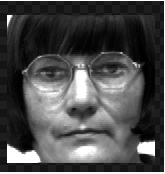
\includegraphics[scale=0.8]{original.png}
     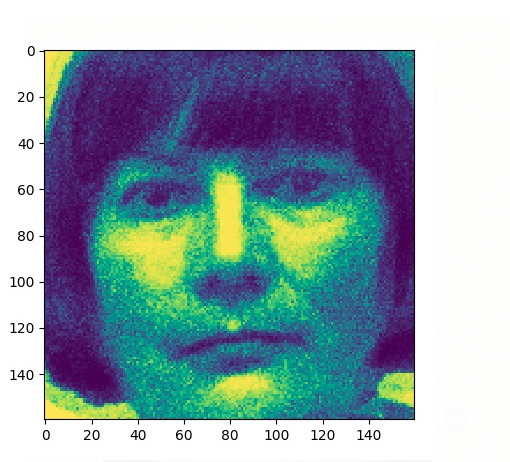
\includegraphics[scale=0.33]{reconstruida.png}
     \caption{Esquerda - Foto original | Direita - Foto reconstruida }
    \end{figure}
    \bibliographystyle{ieeetr}
    \bibliography{sample}
    \end{document}
        
        
        
        
        
        
        
    No newline at end of file
    
    